%--------------------------------------
%ELECTROTECHNIQUE - SCHEMA DE LIAISON A LA TERRE
%--------------------------------------

%utiliser les environnement \begin{comment} \end{comment} pour mettre en commentaire le préambule une fois la programmation appelée dans le document maître (!ne pas oublier de mettre en commentaire \end{document}!)

\begin{comment}

\documentclass[a4paper, 11pt, twoside, fleqn]{memoir}

\usepackage{AOCDTF}

\marqueurchapitre

%lien d'édition des figures Tikz sur le site mathcha.io (rajouter le lien d'une modification effectuée sur la figure tikz avec le nom du modificateur car il n'y a qu'un lien par compte)

%lien éditeur Bruno Douchy : https://www.mathcha.io/editor/zjygnFElSdyhJ72e3zT5ZgqwBT4DKnovswpXn1q

%--------------------------------------
%corps du document
%--------------------------------------

\begin{document} %corps du document
	\openleft %début de chapitre à gauche

\end{comment}

\begin{xltabular}{\textwidth}{l c X c c }
\caption{Différents types de DDR selon les composantes du courant de défaut}\\
\toprule
\thead{Type}		& \thead{Symbole}		& \thead{Caractéristiques}	& \thead{Forme d'onde}		& \thead{Type de charge} \\
\midrule
\endfirsthead %en-tête de la première page du tableau  
\multicolumn{5}{l}{\small\textit{Page précédente}} \\
\midrule %filet de milieu de tableau
\thead{Type}		& \thead{Symbole}		& \thead{Caractéristiques}	& \thead{Forme d'onde}		& \thead{Type de charge} \\
\midrule
\endhead
\midrule %filet de milieu de tableau
\multicolumn{5}{r}{\small\textit{Page suivante}} \\
\endfoot %pied de page de toutes les pages du tableau
\bottomrule
\endlastfoot %pied de page de la dernièredu tableau
Type AC		& \adjustbox{valign=t}{
\includegraphics[height=0.4cm]{type_ac.png}}		& 
\begin{tabitemize}
\item détection des courants alternatifs différentiels\,;
\item utilisation courante en domestique couvrant la plupart des besoin.
\end{tabitemize}
&

\adjustbox{valign=t}{

\tikzset{every picture/.style={line width=0.75pt}} %set default line width to 0.75pt        

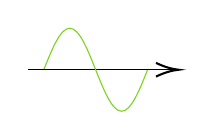
\begin{tikzpicture}[x=0.75pt,y=0.75pt,yscale=-1,xscale=1]
%uncomment if require: \path (0,57); %set diagram left start at 0, and has height of 57

%Straight Lines [id:da2943661507092279] 
\draw    (7.5,25) -- (78,25) ;
\draw [shift={(80,25)}, rotate = 180] [color={rgb, 255:red, 0; green, 0; blue, 0 }  ][line width=0.75]    (10.93,-3.29) .. controls (6.95,-1.4) and (3.31,-0.3) .. (0,0) .. controls (3.31,0.3) and (6.95,1.4) .. (10.93,3.29)   ;
%Shape: Wave [id:dp24323544196681968] 
\draw  [color={rgb, 255:red, 126; green, 211; blue, 33 }  ,draw opacity=1 ] (15,25) .. controls (19.08,14.75) and (22.98,5) .. (27.5,5) .. controls (32.02,5) and (35.92,14.75) .. (40,25) .. controls (44.08,35.25) and (47.98,45) .. (52.5,45) .. controls (57.02,45) and (60.92,35.25) .. (65,25) ;
%Straight Lines [id:da09599799976641754] 
\draw    (7.5,25) -- (30,25) ;
%Straight Lines [id:da7289357219255289] 
\draw    (43.75,25) -- (66.25,25) ;


\end{tikzpicture}}
 &
 
\adjustbox{valign=t}{


\tikzset{every picture/.style={line width=0.75pt}} %set default line width to 0.75pt        

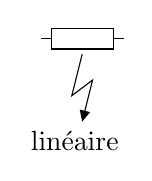
\begin{tikzpicture}[x=0.75pt,y=0.75pt,yscale=-1,xscale=1]
%uncomment if require: \path (0,98); %set diagram left start at 0, and has height of 98

%Straight Lines [id:da7324284340679806] 
\draw    (122.5,17.5) -- (127.5,17.5) ;
%Shape: Rectangle [id:dp18713096911447358] 
\draw   (92.5,12.5) -- (122.5,12.5) -- (122.5,22.5) -- (92.5,22.5) -- cycle ;
%Straight Lines [id:da2214074924221885] 
\draw    (87.5,17.5) -- (92.5,17.5) ;

%Straight Lines [id:da09102665939260723] 
\draw    (107.5,25) -- (102.5,45) -- (112.5,37.5) -- (108.23,54.59) ;
\draw [shift={(107.5,57.5)}, rotate = 284.04] [fill={rgb, 255:red, 0; green, 0; blue, 0 }  ][line width=0.08]  [draw opacity=0] (5.36,-2.57) -- (0,0) -- (5.36,2.57) -- cycle    ;

% Text Node
\draw (81.5,61) node [anchor=north west][inner sep=0.75pt]   [align=left] {linéaire};


\end{tikzpicture}}

  \\
    \addlinespace
  \addlinespace

  
  
  Type A		& \adjustbox{valign=t}{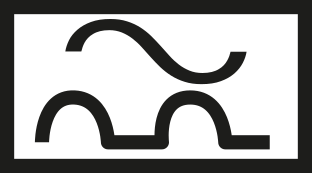
\includegraphics[height=0.4cm]{type_a.png}}		& 
\begin{tabitemize}
\item détection des courants différentiels alternatifs et des courants différentiels continus pulsés\,;
\item utilisation spécifique pour les charges électriques monophasées de type 1.
\end{tabitemize}
&

\adjustbox{valign=t}{




\tikzset{every picture/.style={line width=0.75pt}} %set default line width to 0.75pt        

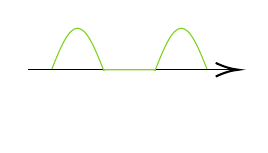
\begin{tikzpicture}[x=0.75pt,y=0.75pt,yscale=-1,xscale=1]
%uncomment if require: \path (0,108); %set diagram left start at 0, and has height of 108

%Shape: Wave [id:dp27700594343461393] 
\draw  [color={rgb, 255:red, 126; green, 211; blue, 33 }  ,draw opacity=1 ] (35,45) .. controls (39.08,34.75) and (42.98,25) .. (47.5,25) .. controls (52.02,25) and (55.92,34.75) .. (60,45) .. controls (64.08,55.25) and (67.98,65) .. (72.5,65) .. controls (77.02,65) and (80.92,55.25) .. (85,45) .. controls (89.08,34.75) and (92.98,25) .. (97.5,25) .. controls (102.02,25) and (105.92,34.75) .. (110,45) ;
%Straight Lines [id:da5910455205676639] 
\draw    (23.75,45) -- (123,45) ;
\draw [shift={(125,45)}, rotate = 180] [color={rgb, 255:red, 0; green, 0; blue, 0 }  ][line width=0.75]    (10.93,-3.29) .. controls (6.95,-1.4) and (3.31,-0.3) .. (0,0) .. controls (3.31,0.3) and (6.95,1.4) .. (10.93,3.29)   ;
%Straight Lines [id:da5095890041059973] 
\draw [color={rgb, 255:red, 126; green, 211; blue, 33 }  ,draw opacity=1 ]   (60,45) -- (85,45) ;
%Shape: Trapezoid [id:dp9576415302257589] 
\draw  [color={rgb, 255:red, 126; green, 211; blue, 33 }  ,draw opacity=1 ] (85,45) -- (84.7,46) -- (60.3,46) -- (60,45) -- cycle ;
%Shape: Rectangle [id:dp7690910497329457] 
\draw  [draw opacity=0][fill={rgb, 255:red, 255; green, 255; blue, 255 }  ,fill opacity=1 ][line width=5.25]  (35,45.5) -- (105,45.5) -- (105,68) -- (35,68) -- cycle ;




\end{tikzpicture}

}
 &
 
 
\adjustbox{valign=t}{



\tikzset{every picture/.style={line width=0.75pt}} %set default line width to 0.75pt        

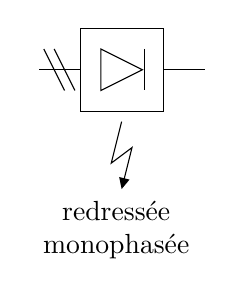
\begin{tikzpicture}[x=0.75pt,y=0.75pt,yscale=-1,xscale=1]
%uncomment if require: \path (0,152); %set diagram left start at 0, and has height of 152

%Straight Lines [id:da2993135281874989] 
\draw    (40,35) -- (30,15) ;
%Straight Lines [id:da1407255659834652] 
\draw    (35,35) -- (25,15) ;
%Straight Lines [id:da0646281171352201] 
\draw    (42.5,25) -- (22.5,25) ;
%Shape: Square [id:dp8095195384599084] 
\draw   (42.5,5) -- (82.5,5) -- (82.5,45) -- (42.5,45) -- cycle ;
%Shape: Boxed Line [id:dp9015036881777688] 
\draw    (73.5,15) -- (73.5,35) ;
%Shape: Triangle [id:dp25930553779074683] 
\draw   (72.5,25) -- (52.5,35) -- (52.5,15) -- cycle ;
%Straight Lines [id:da624315601423471] 
\draw    (62.5,50) -- (57.5,70) -- (67.5,62.5) -- (63.23,79.59) ;
\draw [shift={(62.5,82.5)}, rotate = 284.04] [fill={rgb, 255:red, 0; green, 0; blue, 0 }  ][line width=0.08]  [draw opacity=0] (5.36,-2.57) -- (0,0) -- (5.36,2.57) -- cycle    ;
%Straight Lines [id:da583175718122269] 
\draw    (102.5,25) -- (82.5,25) ;

% Text Node
\draw (17.5,87) node [anchor=north west][inner sep=0.75pt]   [align=left] {\begin{minipage}[lt]{61.699375pt}\setlength\topsep{0pt}
\begin{center}
redressée\\monophasée
\end{center}

\end{minipage}};


\end{tikzpicture}
}

  \\
    \addlinespace
  \addlinespace

  
    Type F		& \adjustbox{valign=t}{
\includegraphics[height=0.4cm]{type_f.png}}		& 
\begin{tabitemize}
\item détection des courants différentiels alternatifs, les courants différentiels continus pulsés et les courants différentiels de fréquences mixtes jusqu'à \SI{1}{\kilo\hertz}\,;
\item utilisation spécifique pour circuits comportant des variateurs de vitesse monophasés.
\end{tabitemize}
&

\adjustbox{valign=t}{
\tikzset{every picture/.style={line width=0.75pt}} %set default line width to 0.75pt        

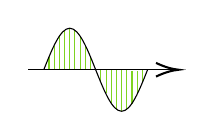
\begin{tikzpicture}[x=0.75pt,y=0.75pt,yscale=-1,xscale=1]
%uncomment if require: \path (0,108); %set diagram left start at 0, and has height of 108

%Straight Lines [id:da8344481258673822] 
\draw [color={rgb, 255:red, 126; green, 211; blue, 33 }  ,draw opacity=1 ]   (47.5,25) -- (47.5,45) ;
%Straight Lines [id:da45734535299498047] 
\draw [color={rgb, 255:red, 126; green, 211; blue, 33 }  ,draw opacity=1 ]   (45,26) -- (45,45) ;
%Straight Lines [id:da4148698837495829] 
\draw [color={rgb, 255:red, 126; green, 211; blue, 33 }  ,draw opacity=1 ]   (42.5,28.5) -- (42.5,44.5) ;
%Straight Lines [id:da9637733631041641] 
\draw [color={rgb, 255:red, 126; green, 211; blue, 33 }  ,draw opacity=1 ]   (37.5,39) -- (37.5,45) ;
%Straight Lines [id:da15505371109761856] 
\draw [color={rgb, 255:red, 126; green, 211; blue, 33 }  ,draw opacity=1 ]   (40,33.5) -- (40,44.5) ;
%Straight Lines [id:da8124028319543418] 
\draw [color={rgb, 255:red, 126; green, 211; blue, 33 }  ,draw opacity=1 ]   (52.5,29) -- (52.5,45) ;
%Straight Lines [id:da9805020896518191] 
\draw [color={rgb, 255:red, 126; green, 211; blue, 33 }  ,draw opacity=1 ]   (50,26) -- (50,45) ;
%Straight Lines [id:da4116431840997269] 
\draw [color={rgb, 255:red, 126; green, 211; blue, 33 }  ,draw opacity=1 ]   (55,34) -- (55,45) ;
%Straight Lines [id:da8823890585871352] 
\draw [color={rgb, 255:red, 126; green, 211; blue, 33 }  ,draw opacity=1 ]   (57.5,39) -- (57.5,45) ;
%Straight Lines [id:da9104778326348498] 
\draw [color={rgb, 255:red, 126; green, 211; blue, 33 }  ,draw opacity=1 ]   (72.5,65) -- (72.5,45) ;
%Straight Lines [id:da36879417192210706] 
\draw [color={rgb, 255:red, 126; green, 211; blue, 33 }  ,draw opacity=1 ]   (75,64) -- (75,45) ;
%Straight Lines [id:da056894793071553984] 
\draw [color={rgb, 255:red, 126; green, 211; blue, 33 }  ,draw opacity=1 ]   (77.5,61.5) -- (77.5,45.5) ;
%Straight Lines [id:da926320044180968] 
\draw [color={rgb, 255:red, 126; green, 211; blue, 33 }  ,draw opacity=1 ]   (82.5,51) -- (82.5,45) ;
%Straight Lines [id:da4802255081072313] 
\draw [color={rgb, 255:red, 126; green, 211; blue, 33 }  ,draw opacity=1 ]   (80,56.5) -- (80,45.5) ;
%Straight Lines [id:da8191961490083182] 
\draw [color={rgb, 255:red, 126; green, 211; blue, 33 }  ,draw opacity=1 ]   (67.5,61) -- (67.5,45) ;
%Straight Lines [id:da2923358818287347] 
\draw [color={rgb, 255:red, 126; green, 211; blue, 33 }  ,draw opacity=1 ]   (70,64) -- (70,45) ;
%Straight Lines [id:da3136693713803336] 
\draw [color={rgb, 255:red, 126; green, 211; blue, 33 }  ,draw opacity=1 ]   (65,56) -- (65,45) ;
%Straight Lines [id:da549046744886196] 
\draw [color={rgb, 255:red, 126; green, 211; blue, 33 }  ,draw opacity=1 ]   (62.5,51) -- (62.5,45) ;

%Shape: Wave [id:dp9341521104203707] 
\draw  [color={rgb, 255:red, 0; green, 0; blue, 0 }  ,draw opacity=1 ] (35,45) .. controls (39.08,34.75) and (42.98,25) .. (47.5,25) .. controls (52.02,25) and (55.92,34.75) .. (60,45) .. controls (64.08,55.25) and (67.98,65) .. (72.5,65) .. controls (77.02,65) and (80.92,55.25) .. (85,45) ;
%Straight Lines [id:da8093364598636541] 
\draw    (27.5,45) -- (98,45) ;
\draw [shift={(100,45)}, rotate = 180] [color={rgb, 255:red, 0; green, 0; blue, 0 }  ][line width=0.75]    (10.93,-3.29) .. controls (6.95,-1.4) and (3.31,-0.3) .. (0,0) .. controls (3.31,0.3) and (6.95,1.4) .. (10.93,3.29)   ;




\end{tikzpicture}

}
 &
 
 
\adjustbox{valign=t}{


\tikzset{every picture/.style={line width=0.75pt}} %set default line width to 0.75pt        

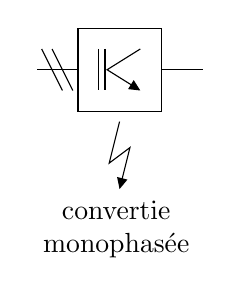
\begin{tikzpicture}[x=0.75pt,y=0.75pt,yscale=-1,xscale=1]
%uncomment if require: \path (0,152); %set diagram left start at 0, and has height of 152

%Straight Lines [id:da2004774518549749] 
\draw    (40,35) -- (30,15) ;
%Straight Lines [id:da28878490688185077] 
\draw    (35,35) -- (25,15) ;
%Straight Lines [id:da28622017833538005] 
\draw    (42.5,25) -- (22.5,25) ;
%Straight Lines [id:da27361779183994883] 
\draw    (62.5,50) -- (57.5,70) -- (67.5,62.5) -- (63.23,79.59) ;
\draw [shift={(62.5,82.5)}, rotate = 284.04] [fill={rgb, 255:red, 0; green, 0; blue, 0 }  ][line width=0.08]  [draw opacity=0] (5.36,-2.57) -- (0,0) -- (5.36,2.57) -- cycle    ;
%Straight Lines [id:da3667194527320474] 
\draw    (102.5,25) -- (82.5,25) ;
%Shape: Square [id:dp27983484657325586] 
\draw   (42.5,5) -- (82.5,5) -- (82.5,45) -- (42.5,45) -- cycle ;
%Shape: Boxed Line [id:dp856307990834614] 
\draw    (52.5,15) -- (52.5,35) ;
%Straight Lines [id:da34232786335443943] 
\draw    (72.5,15) -- (56.5,25) -- (69.96,33.41) ;
\draw [shift={(72.5,35)}, rotate = 212.01] [fill={rgb, 255:red, 0; green, 0; blue, 0 }  ][line width=0.08]  [draw opacity=0] (5.36,-2.57) -- (0,0) -- (5.36,2.57) -- cycle    ;
%Shape: Boxed Line [id:dp1790472061066909] 
\draw    (55.5,15) -- (55.5,35) ;


% Text Node
\draw (18.5,87) node [anchor=north west][inner sep=0.75pt]   [align=left] {\begin{minipage}[lt]{61.699375pt}\setlength\topsep{0pt}
\begin{center}
convertie\\monophasée
\end{center}

\end{minipage}};


\end{tikzpicture}

}

  \\
    \addlinespace
        \addlinespace


      Type B		& \adjustbox{valign=t}{
\includegraphics[height=0.4cm]{type_b.png}}		& 
\begin{tabitemize}
\item détection des courants différentiels alternatifs, les courants différentiels continus pulsés, des courants différentiels de fréquences mixtes jusqu'à \SI{1}{\kilo\hertz} et des courants différentiels continus lisses\,;
\item utilisation spécifique pour circuits comportant des variateurs de vitesse triphasés, un système photovoltaïque, une borne de recharge de véhicule électrique ou encore des équipements médicaux.
\end{tabitemize}
&

\adjustbox{valign=t}{


\tikzset{every picture/.style={line width=0.75pt}} %set default line width to 0.75pt        

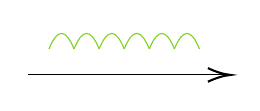
\begin{tikzpicture}[x=0.75pt,y=0.75pt,yscale=-1,xscale=1]
%uncomment if require: \path (0,108); %set diagram left start at 0, and has height of 108

%Straight Lines [id:da7026343722095999] 
\draw    (47.5,87.5) -- (143,87.5) ;
\draw [shift={(145,87.5)}, rotate = 180] [color={rgb, 255:red, 0; green, 0; blue, 0 }  ][line width=0.75]    (10.93,-3.29) .. controls (6.95,-1.4) and (3.31,-0.3) .. (0,0) .. controls (3.31,0.3) and (6.95,1.4) .. (10.93,3.29)   ;
%Shape: Parabola [id:dp4469234992699831] 
\draw  [color={rgb, 255:red, 126; green, 211; blue, 33 }  ,draw opacity=1 ] (69.58,75) .. controls (65.55,65) and (61.52,65) .. (57.5,75) ;
%Shape: Parabola [id:dp10691023078597706] 
\draw  [color={rgb, 255:red, 126; green, 211; blue, 33 }  ,draw opacity=1 ] (81.67,75) .. controls (77.64,65) and (73.61,65) .. (69.58,75) ;
%Shape: Parabola [id:dp9540942461898068] 
\draw  [color={rgb, 255:red, 126; green, 211; blue, 33 }  ,draw opacity=1 ] (93.75,75) .. controls (89.73,65) and (85.7,65) .. (81.67,75) ;
%Shape: Parabola [id:dp6220203064360257] 
\draw  [color={rgb, 255:red, 126; green, 211; blue, 33 }  ,draw opacity=1 ] (105.83,75) .. controls (101.8,65) and (97.77,65) .. (93.75,75) ;
%Shape: Parabola [id:dp4992966008122459] 
\draw  [color={rgb, 255:red, 126; green, 211; blue, 33 }  ,draw opacity=1 ] (117.92,75) .. controls (113.89,65) and (109.86,65) .. (105.83,75) ;
%Shape: Parabola [id:dp01154198803526707] 
\draw  [color={rgb, 255:red, 126; green, 211; blue, 33 }  ,draw opacity=1 ] (130,75) .. controls (125.98,65) and (121.95,65) .. (117.92,75) ;




\end{tikzpicture}

}
 &
 
 
\adjustbox{valign=t}{


\tikzset{every picture/.style={line width=0.75pt}} %set default line width to 0.75pt        

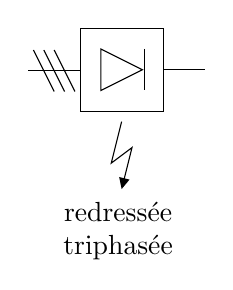
\begin{tikzpicture}[x=0.75pt,y=0.75pt,yscale=-1,xscale=1]
%uncomment if require: \path (0,141); %set diagram left start at 0, and has height of 141

%Straight Lines [id:da4147930693711671] 
\draw    (60,42.5) -- (50,22.5) ;
%Straight Lines [id:da7913487771488718] 
\draw    (55,42.5) -- (45,22.5) ;
%Straight Lines [id:da12782809797617567] 
\draw    (62.5,32.5) -- (37.5,32.5) ;
%Shape: Square [id:dp3051019253176962] 
\draw   (62.5,12) -- (102.5,12) -- (102.5,52) -- (62.5,52) -- cycle ;
%Shape: Boxed Line [id:dp3719227311734635] 
\draw    (93.5,22) -- (93.5,42) ;
%Shape: Triangle [id:dp5734231710257448] 
\draw   (92.5,32) -- (72.5,42) -- (72.5,22) -- cycle ;
%Straight Lines [id:da20189459286959577] 
\draw    (82.5,57) -- (77.5,77) -- (87.5,69.5) -- (83.23,86.59) ;
\draw [shift={(82.5,89.5)}, rotate = 284.04] [fill={rgb, 255:red, 0; green, 0; blue, 0 }  ][line width=0.08]  [draw opacity=0] (5.36,-2.57) -- (0,0) -- (5.36,2.57) -- cycle    ;
%Straight Lines [id:da8309944422064088] 
\draw    (122.5,32) -- (102.5,32) ;
%Straight Lines [id:da522665354082454] 
\draw    (50,42.5) -- (40,22.5) ;

% Text Node
\draw (47.5,94.5) node [anchor=north west][inner sep=0.75pt]   [align=left] {\begin{minipage}[lt]{48.078125pt}\setlength\topsep{0pt}
\begin{center}
redressée\\triphasée
\end{center}

\end{minipage}};


\end{tikzpicture}


}

  \\
  \addlinespace
  
\end{xltabular}


%\end{document}

